\documentclass{beamer}

\usepackage{verbatim}
\usepackage{xcolor} % See documentation PDF at http://www.ctan.org/pkg/xcolor
\definecolor{darkgreen}{rgb}{0,0.3,0}
\definecolor{lightgrey}{rgb}{0.65,0.65,0.65}
\usepackage{tikzsymbols}


\setbeamertemplate{section in toc}[sections numbered]
\setbeamertemplate{subsection in toc}[subsections numbered]
\setbeamertemplate{subsubsection in toc}[subsubsections numbered]
\usetheme{Singapore}
\setbeamertemplate{navigation symbols}{}
\setbeamertemplate{footline}{%
\vspace{0.0em}%
\hspace{0.5em}%
{\color[rgb]{.1,.1,.1} \insertframenumber{}~/~\inserttotalframenumber}
}

\newcommand{\code}[1]{{\color{darkgreen}\texttt{#1}}}
\newcommand{\detail}[1]{{\color{lightgrey}\small{}#1}}


\begin{document}

\title{Formal Models of Language \\[1.5em]
 
\includegraphics[width=0.5\textwidth]{images/kitten_string_flickr_albaraa.jpg} \\[-1.0em]
 %\small{Possibilities} \\[1.0em]
 %LT1 \\[1.0em]
 }
\author{\href{http://jon.dehdari.org}{Jon Dehdari}}
\frame{\titlepage}

\begin{frame}{Introduction}
Hi!
\end{frame}

% Formal language
\begin{frame}{Formal Languages}
\begin{block}{}
\begin{itemize}
	\item Once Upon a Time...
	\pause
	\item Mathematicians started to think about language...
	\pause
	\item They used ideas from logic to represent linguistic objects...
	\pause
	\item They had a craaaazy idea... \\
	\pause
	\begin{center}
	
\includegraphics[width=0.6\textwidth]{images/doc_brown_strings.jpg}
	\end{center}
\end{itemize}
\end{block}
\end{frame}


\begin{frame}{Strings}
\begin{block}{What's a String?}
\begin{itemize}
	\item A \textbf{string} in this context is just a sequence of words
	\pause
	\item A \textbf{formal language} ($L$) is a subset of all the possible strings
	\pause
	\item An \textbf{vocabulary} ($\Sigma$, also sometimes called \textit{alphabet}) here is a set of all the words in the language
	\pause
	\item Words here don't need to correspond to words used for natural languages
	\pause
	\item For example, this set:\\
	\begin{center}
	{\LARGE \{ \Smiley[][cyan], \Springtree, \Snowman \}}\\
	\end{center}
	is a perfectly valid vocabulary for a formal language. \pause But we usually use boring symbols like \{a, b, c\}
	\pause
	\item {\scriptsize (Similar to musical/poetic form analysis)}
\end{itemize}
\end{block}
\end{frame}


% Formal grammar: grammar, automaton
\begin{frame}{Formal Grammar}
\begin{block}{}
\begin{itemize}
	\item A formal grammar is a way of telling what a valid string is in a formal language
	\item Formal grammars can also \textbf{generate} valid strings
	\pause
% weak & strong generative capacity
	\item If two different grammars can generate/accept the same formal languages, then they have the same \textbf{weak generative capacity}
	\pause
	\item If two different grammars can generate/accept the same structures as well, then they have the same \textbf{strong generative capacity}
\end{itemize}
\end{block}
\end{frame}


% Chomsky Hierarchy
\begin{frame}{Formal Language Hierarchy}
\begin{center}
\begin{tabular}{|ll|}
\hline
& Formal Language \\
\hline
\hline
& Non-Turing-acceptable\\
\hline
0: & \bf Recursively enumerable \\
\hline
& Recursive/\,Decidable \\
\hline
1: & Context-sensitive \\
\hline
& Indexed \\
\hline
& \bf Mildly context-sensitive \\
\hline
2: & \bf Context-free \\
\hline
& \bf Deterministic context-free \\
\hline
3: & \bf Regular \\
\hline
& \bf Finite \\
\hline
\end{tabular}
\end{center}
\pause
\footnotesize{This is extended from the older \textit{Chomsky hierarchy}. \pause We'll discuss the ones in boldface, as they're relevant to natural languages.}
\end{frame}


% applications of knowing this stuff
\begin{frame}{Why is this Stuff Relevant??}
\begin{block}{}
\begin{itemize}
	\item Knowing what types of formal languages a grammar/automaton can generate \& accept will give you an idea of what phenomena in natural languages that they can handle
	\pause
	\item For example: long-distance dependencies, complex reordering in machine translation, reduplication, etc.
	\pause
	\item You can also get an idea of how fast or slow it will take for a computer (or human) to process sequential stuff (like natural language!)
\end{itemize}
\end{block}
\end{frame}


\begin{frame}{Finite Languages}
\begin{block}{}
\begin{itemize}
	\item In a finite language, there are a finite (ie not infinite) number of valid \textit{sentences}.
	\item Time: constant (through hash-table lookup)
	\item Memory: constant (duh)
	\pause
	\item For natural language, this would correspond to having a finite number of possible sentences
\end{itemize}
\end{block}
\end{frame}


\begin{frame}{Are Natural Languages Finite??!!}
\begin{block}{}
\begin{itemize}
	\item It sounds crazy to think that you could ever list all of the possible sentences of a natural language
	\pause
	\item Really, really crazy
	\pause
	\item But...
	\pause
	\item There's a big difference between a really large number and infinity
	\pause
	\item {\small If a natural language has a vocabulary of, say, 100 million words ...}
	\pause
	\item And a sentence can have, say, up to 10,000 words in it, ...
	\pause
	\item Then there would be $10^{80,000}$ possible sentences
	\pause
	\item This number sounds way too big to be practical for either humans or computers to deal with!
	\pause
	\item But it's much smaller than infinity.
	\pause
	\item Much much smaller.
	\pause
	\item \tiny{\href{http://people.umass.edu/~partee/726_04/lectures/Is_Language_Infinite.pdf}{(There's more discussion on the interwebs if you're interested)}}
\end{itemize}
\end{block}
\end{frame}


% Regular language: fixed history: linear time, constant memory.  Regular grammars can actually do alot
\begin{frame}{Regular Languages}
\begin{block}{}
\begin{itemize}
	\item Ok, so maybe for now it's too difficult to list all possible sentences
	\item Let's assume that the vocabulary ($\Sigma$) is still fixed (or finite), but we can generate an infinite number of sentences from this fixed vocab
	\item Regular grammars have a fixed-length history, so they're limited in the types of long-distance phenomena they can handle
	\pause
	\item Processing regular languages can be done in linear time \detail{($\mathcal{O}(n)$)}, with a constant size of memory \detail{($\mathcal{O}(1)$)}
\end{itemize}
\end{block}
\end{frame}


% DCF lang: full history, as long as unambiguous: linear time, log^2(n) memory
\begin{frame}{Deterministic Context-Free Languages}
\begin{block}{}
\begin{itemize}
	\item Deterministic context-free (DCF) languages include longer-distance phenomena
	\item DCF grammars have a full-length history, as long as there's no ambiguity (ie.\ it can't backtrack)
	\pause
	\item Processing DCF languages can be done in linear time \detail{($\mathcal{O}(n)$)}, with linear memory usage \detail{($\mathcal{O}(n)$)}
\end{itemize}
\end{block}
\end{frame}


\begin{frame}{Context-Free Languages}
\begin{block}{}
\begin{itemize}
	\item Context-free languages include phenomena like center embedding
	\item For example ...
	%% (use whiteboard for now to draw example)
	\pause
	\item Context-free grammars have a full-length history, and they can backtrack for ambiguous sentences
	\pause
	\item Processing DCF languages can be done in about cubic time \detail{($\mathcal{O}(n^3)$)}, with linear memory usage \detail{($\mathcal{O}(n)$)}
\end{itemize}
\end{block}
\end{frame}


% MCS lang: same, allows full reduplication (cross-serial deps) and a^n b^n c^n d^n: n^6 time. TAG, CCG, LIG, Head Grammars, 
\begin{frame}{Mildly Context-Sensitive Languages}
\begin{block}{}
\begin{itemize}
	\item Mildly context-sensitive (MCS) languages include phenomena like reduplication and cross-serial dependencies.
	\item Example:\pause
	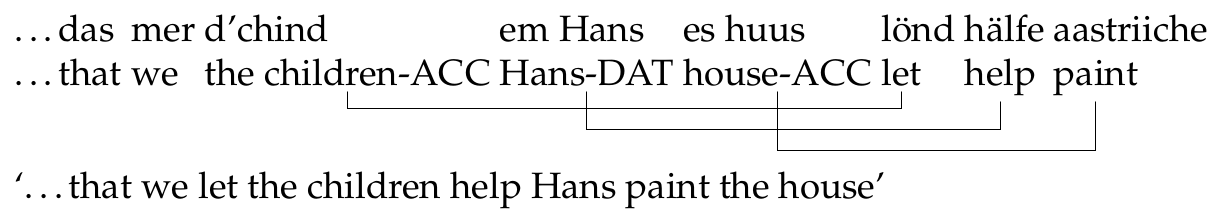
\includegraphics[width=0.80\textwidth]{images/swiss_cross_serial_deps.png}
	%% (use whiteboard for now to draw example)
	\pause
	\item Processing MCS languages can be done in $\mathcal{O}(n^6)$ time, with quadratic memory usage \detail{($\mathcal{O}(n^2)$)}
	\pause
	\item Some grammar formalisms that can handle MCS languages include:
	\begin{itemize}
		\item Tree Adjoining Grammar (TAG)
		\item Combinatory Categorial Grammar (CCG)
		\item Linear Indexed Grammars (LIG)
		\item Head Grammars (HG)
	\end{itemize}
\end{itemize}
\end{block}
\end{frame}


% Recursively enumerable langs: allows any string that a computer (eg. Turing machine, untyped \lambda calculus, MLP) can generate
\begin{frame}{Recursively Enumerable Languages}
\begin{block}{}
\begin{itemize}
	\item Recursively enumerable languages allow any string that a computer (or equivalent device) can generate/accept
	\item There's no guarantee that the computer will ever stop processing the sentence \detail{$\mathcal{O}(\infty)$}
	\item Essentially any word can occur in any place in the sentence
	\pause
	\item Some grammar formalisms that allow recursively enumerable languages include:
	\begin{itemize}
		\item Chomskyan grammars (due to transformations / moves)
		\item Lexical Functional Grammar (LFG)
		\item Head-driven Phrase Structure Grammar (HPSG)
	\end{itemize}
	\pause
	\item Note that these grammar formalisms can place some restrictions on word order, but they still accept/generate recursively enumerable languages. \pause How is that so? \pause Additional grammar rules can work around such restrictions to accept/generate the string.
\end{itemize}
\end{block}
\end{frame}



% \begin{frame}{}
% \begin{block}{}
% \begin{itemize}
% 	\item 
% 	\item 
% 	\item 
% \end{itemize}
% \end{block}
% \end{frame}


\end{document}
